\documentclass[11pt]{article}
\usepackage[utf8]{inputenc}
\usepackage{graphicx}
\graphicspath{ {images/} }
\usepackage{amsmath}

\title{Coursework 1 – Transient Conduction}
\author{Adam Duncan}
\date{\today}

\begin{document}

\maketitle

\section{\emph{Part A: Using lumped capacitance}}
\subsection{Assumptions}
\begin{itemize}
	\item Internal temperature of the steel ball is uniform at any time t.
	\item No change in water temperature
	\item No heat transfer by radiation
	\item Material is standard carbon steel
	\item Material properties constant (taken at average temperature $T = 469 ^{o}C$)
\end{itemize}
\subsection{Schematic}
\begin{figure}[h]
	\centering
	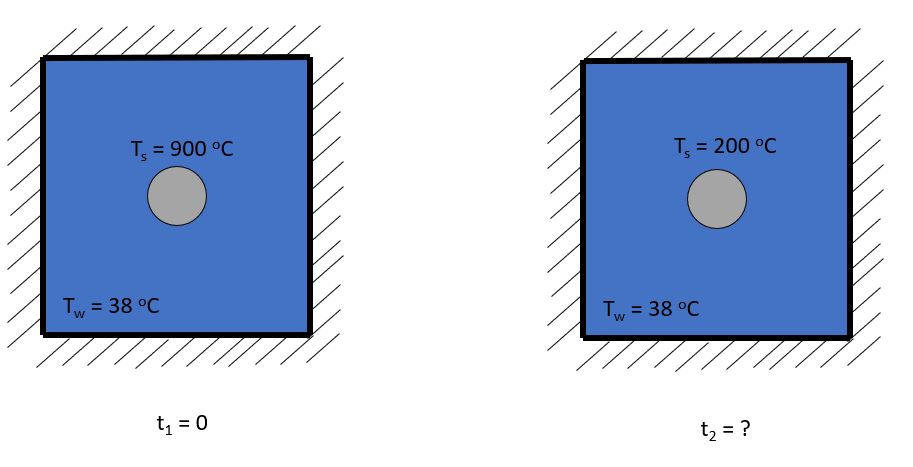
\includegraphics[width=0.85\textwidth]{part_a_fig}
	\caption{Part A schematic at initial and final state.}
	\label{fig:schem_a}
\end{figure}
\subsection{Analysis}
Energy balance for closed system gives the following equation.
\begin{equation}\label{eqn_1}
	\stackrel{.}{Q} = hA(T_{c}-T_{f}) = C_{p}\rho V \frac{dT_{c}}{dt}
\end{equation}

Where $\stackrel{.}{Q}$ is energy flow [$W$], $h$ is the heat transfer coefficient [$W/m^{2}K$], $A$ is the surface area between the ball and water [$m^{2}$], $T_{c}$ is the temperature of the steel ball [$^{o}C$], $T_{f}$ is the temperature of the water [$^{o}C$], $C_{p}$ is the specific heat capacity [$J/mK$], $\rho$ is the density of the steel ball[$kg/m^{3}$], $V$ is the volume of the steel ball [$m^3$] and $t$ is the time [$s$].
\newline

Rearranging to separate the variables gives.
\begin{equation}\label{key}
	\frac{1}{T_{c}-T_{f}} dT_{c} = \frac{hA}{C_{p}\rho V}dt
\end{equation}
Which integrates to give.
\begin{equation}\label{key}
	\ln{(\frac{T_{c1}-T_{f}}{T_{c2}-T_{f}})} =  \frac{hA}{C_{p}\rho V}(t_{2}-t_{1})
\end{equation}
Where $t_{i}$ is the time [s] at state i.
\begin{equation}
	Bi = \frac{h L_{c}}{k}
\end{equation}
Where $h$ is conductivity [W/mK]
\begin{equation}
	t=\frac{f_{0} \rho C_{p} R^{2}}{k}
\end{equation}
\section{\emph{Part B: Lumped capacitance justification}}

\section{\emph{Part C: Transient conduction}}

\section{\emph{Part D: Non-infinite water bath}}

\section{\emph{Part E: Equilibrium temperature}}
\end{document}
